\documentclass[a4paper]{article}
\addtolength{\hoffset}{-2.25cm}
\addtolength{\textwidth}{4.5cm}
\addtolength{\voffset}{-3.25cm}
\addtolength{\textheight}{5cm}
\setlength{\parskip}{0pt}
\setlength{\parindent}{0in}

\usepackage[square,sort,comma,numbers]{natbib}
\usepackage{blindtext} % Package to generate dummy text
\usepackage{charter} % Use the Charter font
\usepackage[utf8]{inputenc} % Use UTF-8 encoding
\usepackage{microtype} % Slightly tweak font spacing for aesthetics
\usepackage{amsthm, amsmath, amssymb} % Mathematical typesetting
\usepackage{float} % Improved interface for floating objects
\usepackage{hyperref} % For hyperlinks in the PDF
\usepackage{graphicx, multicol} % Enhanced support for graphics
\usepackage{xcolor} % Driver-independent color extensions
\usepackage{pseudocode} % Environment for specifying algorithms in a natural way
\usepackage[mmddyy]{datetime} % Uses YEAR-MONTH-DAY format for dates

\usepackage{fancyhdr} % Headers and footers
\pagestyle{fancy} % All pages have headers and footers
\fancyhead{}\renewcommand{\headrulewidth}{0pt} % Blank out the default header
\fancyfoot[L]{} % Custom footer text
\fancyfoot[C]{} % Custom footer text
\fancyfoot[R]{\thepage} % Custom footer text
\newcommand{\note}[1]{\marginpar{\scriptsize \textcolor{red}{#1}}} % Enables comments in red on margin

\DeclareMathOperator*{\argmin}{arg\,min}

%----------------------------------------------------------------------------------------

\newcommand{\yourname}{Balthazar Neveu}
\newcommand{\youremail}{balthazarneveu@gmail.com}
\newcommand{\assignmentnumber}{6}

\begin{document}

\fancyhead[C]{}
\hrule \medskip
\begin{minipage}{0.295\textwidth} 
\raggedright
\footnotesize
\yourname \hfill\\
\youremail
\end{minipage}
\begin{minipage}{0.4\textwidth} 
\centering 
\large 
Lab session \# \assignmentnumber\\ 
\normalsize 
ALTEGRAD 2023\\ 
\end{minipage}
\begin{minipage}{0.295\textwidth} 
\raggedleft
\today\hfill\\
\end{minipage}
\medskip\hrule 
\bigskip


\section*{Code}

More info:
\href{https://github.com/balthazarneveu/MVA23_ALTEGRAD/#readme}{MVA ALTEGRAD Balthazar Neveu on Github}

\section{Section 1: Graph-level classification}
\subsection*{Question 1: $\mathbb{E}(d)^{p=0.2} = 4.8$ and $\mathbb{E}(d)^{p=0.4} = 9.6$}
We denote a graph $G = (V, E)$ where $v_i \in V$ denote the vertices or nodes and $E$ are the edges.
\subsubsection*{Preliminary remark : Overall statistics of edges}

The total number of undirected edges when the graph is dense is ${n\choose 2} =\frac{n(n-1)}{2}$
When $n=25$, the densest graph will have 300 edges (when $p=1$).
The Erdős–Rényi has in average $p * {n=25 \choose 2}$ edges.

\subsubsection*{Distribution of the degree $d$}
For a given node $v{i}$, the probability to be connected to $v_j$ where $i \neq j$ is a
Bernoulli distribution.
$$\mathbb{P}[(v_{i},v_{j}) \in E] \sim \mathbb{B}(p)$$ 
Degree of edge $v_{i}$ is the number of all connected nodes (number of edges).
It therefore follows a Binomial distribution. 
The maximum number of edges is $n-1$ ($d \leq n-1$)
The expectation of the degree $d$ is:
$$\mathbb{E}(d) = (n-1).p$$

\textit{Note: Computing the degree is equivalent to counting the number of flipped coins with a tail (1 toss of a coin with probability $p$ of having a tail is equivalent 
to get a connected 1 edge)}

\textit{Note: Obviously, degenerate case when $p=1$, the degree reaches the maximum as we'd expect.}

\subsubsection*{Numerical application}
$$\mathbb{E}(d)^{p=0.2} = 24*0.2 = 4.8$$
$$\mathbb{E}(d)^{p=0.4} = 24*0.4 = 9.6$$

\subsection*{Question 2: Readout operator}
Readout functions shall reduce the graph's "spatial dimension" (they're the equivalent for graph to global pooling operation for image and signal processing).
Therefore, there are a certain amount of guideline for the readout operators:
\begin{itemize}
    \item permutation invariant
    \item size agnostic
\end{itemize} 
Fully connected layers do not like good "Readout" functions.

The weight matrix of a fully connected layer is fixed, so the number of nodes is fixed.

Assume for a minute you'd train a fully connected layer to replace the readout function. If you trained it on $G_1, G_2, G_3$ which have a different sizes number of nodes,
you could use a weight matrix of size determined by the graph which most nodes ($G_2$ has $|V_{G_2}|=4$ nodes here).
Weight matrix would have a fixed size $(|V_{G_2}|*h_{\text{in}}, h_{\text{out}} )$ and you'd have to pad the input vectors with zeros when there are not enough nodes.

This simply feels wrong: we could assume you'd pad with zeros if a new test graph has more nodes or remove some nodes when there are less nodes.

Last but not least, a fully connected layer is not permutation invariant (shuffle input features of a linear layer and you get a different result).

\textit{Closing remark:}
The case where it would make sense is for instance if the graph nodes are always ordered the same way, basically meaning that there's an underlying geometric structure.

One could think of MRI connectivity between areas of the brain where the nodes are always localized at the same spatial location using an atlas of "standardized areas" like the Harvard-Oxford brain atlas.
Brain MRI seem to be standardized this way and this introduces hard constraints in the nature of the data.


It seems like such readout is not such a bad idea for some special graph-level problems (drug discovery mentioned \href{https://github.com/davidbuterez/gnn-neural-readouts}{Neural readouts} this is an active area of research.)

\subsection*{Task 3}
\begin{verbatim}
Epoch: 0191 loss_train: 0.3165 acc_train: 85.39% time: 0.0434s
Optimization finished!
loss_test: 0.2615 acc_test: 88.89% time: 0.0466s
\end{verbatim}


\section*{Section 2: Graph Neural Networks expressiveness}
\section*{Question 3: influence of readout and aggregation functions while discriminating Cycle graphs with GNN}
In the following, $n > 2$ denotes the number of nodes in the cycle graph $C_{n}$.
\begin{itemize}
    \item \textit{neighbor aggregation = mean},\textbf{readout= mean: same features} (same graph description $\forall{n}$)
    \item \textit{neighbor aggregation = sum}, \textbf{readout= mean: same features} (same graph description $\forall{n}$)
    \item \textit{neighbor aggregation = mean, readout= sum}: different features
    \item \textit{neighbor aggregation = sum, readout= sum}: different features
\end{itemize}



Using the mean readout gives similar characteristics describing all the different cycle graphs.
The expressiveness of the GNN increases with the sum readout which leads to different representation when $n$ varies.
Using the mean or sum in neighbor aggregation does not change anything in the resulting representation (simply a scaling factor). We cannot make generalities

An handwavy explanation is that the sum in the readout allows "counting" features (here the underlying count refers to the number of nodes).

Let's break things down.

\begin{itemize}
    \item $X$ input are all ones.
    \item In the message passing, $MP(A, X)$ 
        \subitem - projected inputs features will be mapped to the same vectors $X.W_{0}$ has all equal rows.
        \subitem - since all nodes in a cycle graph have 2 neighbors
        \subitem - sum aggregation: $A.(X.W_{0}) = 2(X.W_{0}$) in this special case... will also have all equal rows.
        \subitem - mean aggregation: $D^{-1}.A.(X.W_{0}) = (X.W_{0}$) will also have all equal rows.
        \subitem - by extension $Z^{0} = ReLu(MP(A, X))$ has equal rows for the sum or mean aggregation
    \item most importantly, $\forall{n} > 2$ the rows of $Z{0}$ are even the same no matter the length of the cycle graph.
    \item The same reasoning goes for $Z^{1}$, let's define $z^{1}$ a single row of $Z^{1}$.
    \item Readout:
        \subitem  \textbf{Sum readout($Z^1$)}: sum over all the rows which are equal. We end up with $n*u$
        \subitem  \textbf{Average readout($Z^1$)}: average over all the rows which are equal. We end up with a single row of $u$, no matter the length $n$
\end{itemize}
Below is a quick numerical validation of the proportionality in $n$ for the sum readout.

\break

We remark the proportionality property for the sum Readout.($Z^{1}_{G} \propto{n}$)


\begin{figure}[ht]
    \centering
    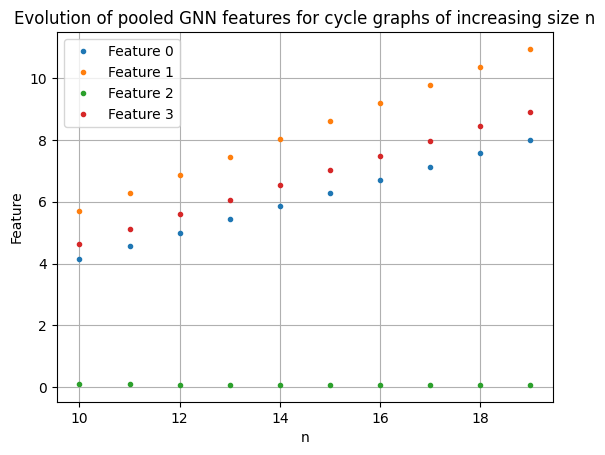
\includegraphics[width=0.6\textwidth]{figures/features_evolution.png}
    \caption{Evolution of graph descriptors using the sum readout. We can validate the linear evolution in $n$ }
    \label{fig:node_embeddings}
\end{figure}


\begin{verbatim}
neighbor_aggr='sum', readout='sum'
[
    [ 4.146614    5.709204    0.09333157  4.6471424 ]
    [ 4.5737143   6.290244    0.09161585  5.1209064 ]
    [ 5.000814    6.8712826   0.08990037  5.594671  ]
    [ 5.4279146   7.452322    0.08818489  6.068435  ]
    [ 5.8550153   8.033361    0.08646905  6.542199  ]
    [ 6.282116    8.614401    0.08475303  7.015964  ]
    [ 6.709216    9.195441    0.08303796  7.4897275 ]
    [ 7.1363163   9.77648     0.08132147  7.963493  ]
    [ 7.563416   10.357518    0.07960581  8.437258  ]
    [ 7.9905176  10.938558    0.07789027  8.911022  ]
]      
\end{verbatim}

\subsection*{Task 11}
\begin{verbatim}
neighbor_aggr='sum', readout='sum'
G1 representation: [-2.1668684  4.630975  -3.4005415  1.7028651]
G2 representation: [-2.1668684  4.630975  -3.4005415  1.7028651]
\end{verbatim}
Same representation although the graphs are different (not isomorphic!).
We note that $G^2 =C^6$ being a cycle graph, we shown in question 3 that it will have a representation $z^{1}_{C^6} = 2 z^{1}_{C^3}$..
Now we nottice that $G^{1} = C^3 \cup C^3$ (2 connected components $C^3$). The readout will sum the features of these 2 graphs,
ending up with $z^{1}_{C^6} = 2. z^{1}_{C^3}$.
So this was expected.

\break
\subsection*{Question 4}
Example 1 and 2 are similar to the trick used in task 11 although they're different.

\subsubsection*{Example 0}
$G^1$ is a square with 4 nodes, $G^2$ is made 2 connected components made of pairs (path of 2 nodes $P^2$) so no cycle involved in one of them 
\begin{itemize}
    \item $G^1 =C^4$ as shown in \ref{fig:c4}
    \item $G^2 =P^2 \cup P^2$ shown in \ref{fig:2k2}
\end{itemize} 
are not isomorphic but their GNN representations are the same.

\begin{verbatim}
G1 representation: [-2.7711809  2.5115702  2.4466345  2.0798717]
G2 representation: [-2.7711809  2.5115702  2.4466345  2.0798717]
\end{verbatim}

\begin{figure}[ht]
    \centering
    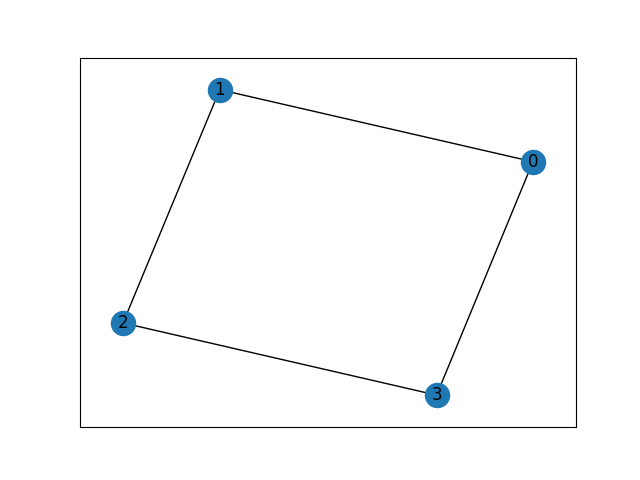
\includegraphics[width=0.6\textwidth]{figures/c4.png}
    \caption{$G^1 =C^4$}
    \label{fig:c4}
\end{figure}

\begin{figure}[ht]
    \centering
    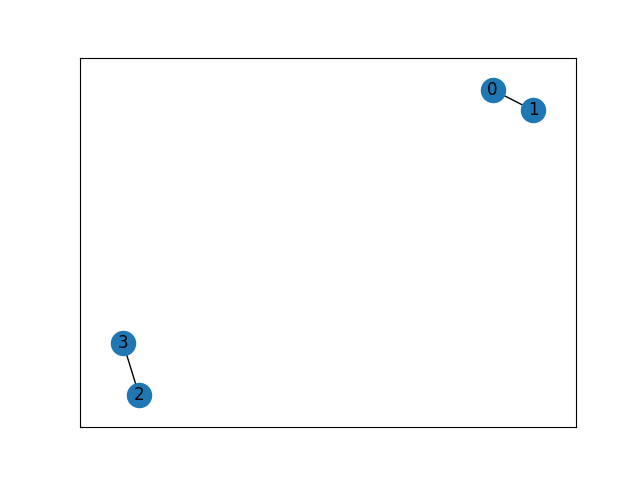
\includegraphics[width=0.6\textwidth]{figures/2k2.png}
    \caption{$G^2 =P^2 \cup P^2$}
    \label{fig:2k2}
\end{figure}

\break

\subsubsection*{Example 1}
\begin{itemize}
    \item $G^1 =C^5 \cup C^7$ shown in \ref{fig:c5_u_c7}
    \item $G^2 =C^{12}$ shown in \ref{fig:c12}
\end{itemize} 
are not isomorphic but their GNN representation are the same.

\begin{verbatim}
    G1 representation: [6.511315   1.9150434  0.20283365 3.483223  ]
    G2 representation: [6.511315   1.9150434  0.20283365 3.483223  ]
\end{verbatim}

\begin{figure}[ht]
    \centering
    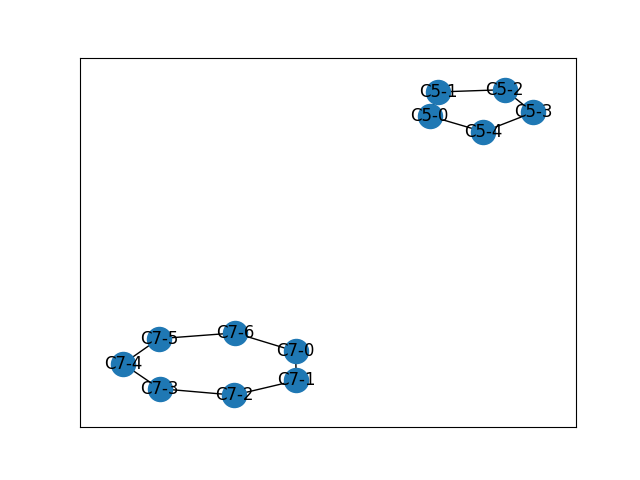
\includegraphics[width=0.6\textwidth]{figures/c5_u_c7.png}
    \caption{$G^1 =C^5 \cup C^7$}
    \label{fig:c5_u_c7}
\end{figure}

\begin{figure}[ht]
    \centering
    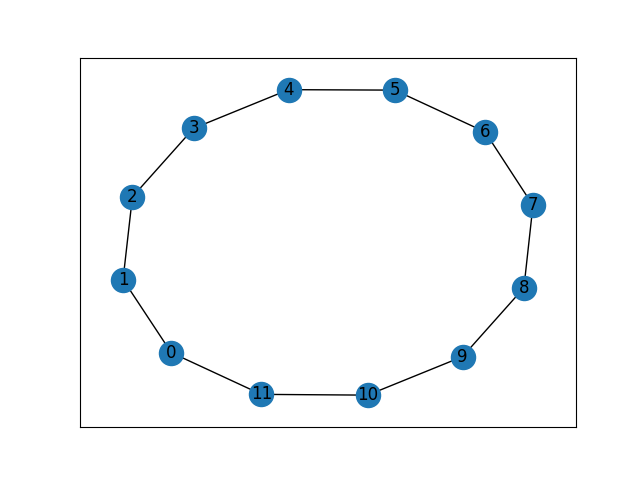
\includegraphics[width=0.6\textwidth]{figures/c12.png}
    \caption{$G^2 =C^{12}$}
    \label{fig:c12}
\end{figure}
\break
\subsubsection*{Example 2}
$G^1 =C^4 \cup C^4$ shown in \ref{fig:c4_u_c4} and $G^2 =C^8$ shown in \ref{fig:c8} are not isomorphic but their GNN representation are the same.
\begin{figure}[ht]
    \centering
    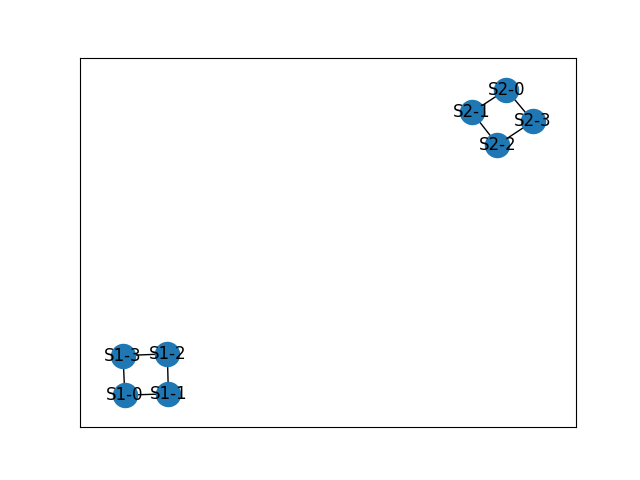
\includegraphics[width=0.6\textwidth]{figures/C4_u_C4.png}
    \caption{$G^1 =C^4 \cup C^4$}
    \label{fig:c4_u_c4}
\end{figure}

\begin{figure}[ht]
    \centering
    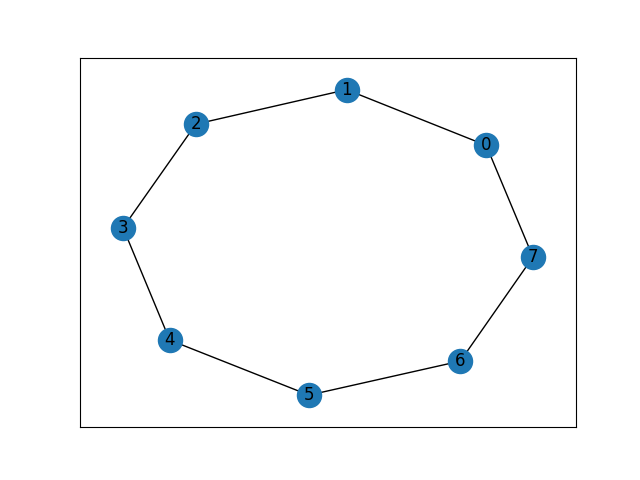
\includegraphics[width=0.6\textwidth]{figures/C8.png}
    \caption{$G^2 =C^8$}
    \label{fig:c8}
\end{figure}

\begin{verbatim}
G1 representation: [-0.3330682 -1.2836217  4.3689184  2.9682496]
G2 representation: [-0.3330682 -1.2836217  4.3689184  2.9682496]
These are the same although the graphs are not isomorphic    
\end{verbatim}
% \bibliographystyle{plain}
% \bibliography{references}

\end{document}